% Options for packages loaded elsewhere
\PassOptionsToPackage{unicode}{hyperref}
\PassOptionsToPackage{hyphens}{url}
\PassOptionsToPackage{dvipsnames,svgnames,x11names}{xcolor}
%
\documentclass[
  letterpaper,
  DIV=11,
  numbers=noendperiod]{scrartcl}

\usepackage{amsmath,amssymb}
\usepackage{iftex}
\ifPDFTeX
  \usepackage[T1]{fontenc}
  \usepackage[utf8]{inputenc}
  \usepackage{textcomp} % provide euro and other symbols
\else % if luatex or xetex
  \usepackage{unicode-math}
  \defaultfontfeatures{Scale=MatchLowercase}
  \defaultfontfeatures[\rmfamily]{Ligatures=TeX,Scale=1}
\fi
\usepackage{lmodern}
\ifPDFTeX\else  
    % xetex/luatex font selection
\fi
% Use upquote if available, for straight quotes in verbatim environments
\IfFileExists{upquote.sty}{\usepackage{upquote}}{}
\IfFileExists{microtype.sty}{% use microtype if available
  \usepackage[]{microtype}
  \UseMicrotypeSet[protrusion]{basicmath} % disable protrusion for tt fonts
}{}
\makeatletter
\@ifundefined{KOMAClassName}{% if non-KOMA class
  \IfFileExists{parskip.sty}{%
    \usepackage{parskip}
  }{% else
    \setlength{\parindent}{0pt}
    \setlength{\parskip}{6pt plus 2pt minus 1pt}}
}{% if KOMA class
  \KOMAoptions{parskip=half}}
\makeatother
\usepackage{xcolor}
\setlength{\emergencystretch}{3em} % prevent overfull lines
\setcounter{secnumdepth}{-\maxdimen} % remove section numbering
% Make \paragraph and \subparagraph free-standing
\ifx\paragraph\undefined\else
  \let\oldparagraph\paragraph
  \renewcommand{\paragraph}[1]{\oldparagraph{#1}\mbox{}}
\fi
\ifx\subparagraph\undefined\else
  \let\oldsubparagraph\subparagraph
  \renewcommand{\subparagraph}[1]{\oldsubparagraph{#1}\mbox{}}
\fi

\usepackage{color}
\usepackage{fancyvrb}
\newcommand{\VerbBar}{|}
\newcommand{\VERB}{\Verb[commandchars=\\\{\}]}
\DefineVerbatimEnvironment{Highlighting}{Verbatim}{commandchars=\\\{\}}
% Add ',fontsize=\small' for more characters per line
\usepackage{framed}
\definecolor{shadecolor}{RGB}{241,243,245}
\newenvironment{Shaded}{\begin{snugshade}}{\end{snugshade}}
\newcommand{\AlertTok}[1]{\textcolor[rgb]{0.68,0.00,0.00}{#1}}
\newcommand{\AnnotationTok}[1]{\textcolor[rgb]{0.37,0.37,0.37}{#1}}
\newcommand{\AttributeTok}[1]{\textcolor[rgb]{0.40,0.45,0.13}{#1}}
\newcommand{\BaseNTok}[1]{\textcolor[rgb]{0.68,0.00,0.00}{#1}}
\newcommand{\BuiltInTok}[1]{\textcolor[rgb]{0.00,0.23,0.31}{#1}}
\newcommand{\CharTok}[1]{\textcolor[rgb]{0.13,0.47,0.30}{#1}}
\newcommand{\CommentTok}[1]{\textcolor[rgb]{0.37,0.37,0.37}{#1}}
\newcommand{\CommentVarTok}[1]{\textcolor[rgb]{0.37,0.37,0.37}{\textit{#1}}}
\newcommand{\ConstantTok}[1]{\textcolor[rgb]{0.56,0.35,0.01}{#1}}
\newcommand{\ControlFlowTok}[1]{\textcolor[rgb]{0.00,0.23,0.31}{#1}}
\newcommand{\DataTypeTok}[1]{\textcolor[rgb]{0.68,0.00,0.00}{#1}}
\newcommand{\DecValTok}[1]{\textcolor[rgb]{0.68,0.00,0.00}{#1}}
\newcommand{\DocumentationTok}[1]{\textcolor[rgb]{0.37,0.37,0.37}{\textit{#1}}}
\newcommand{\ErrorTok}[1]{\textcolor[rgb]{0.68,0.00,0.00}{#1}}
\newcommand{\ExtensionTok}[1]{\textcolor[rgb]{0.00,0.23,0.31}{#1}}
\newcommand{\FloatTok}[1]{\textcolor[rgb]{0.68,0.00,0.00}{#1}}
\newcommand{\FunctionTok}[1]{\textcolor[rgb]{0.28,0.35,0.67}{#1}}
\newcommand{\ImportTok}[1]{\textcolor[rgb]{0.00,0.46,0.62}{#1}}
\newcommand{\InformationTok}[1]{\textcolor[rgb]{0.37,0.37,0.37}{#1}}
\newcommand{\KeywordTok}[1]{\textcolor[rgb]{0.00,0.23,0.31}{#1}}
\newcommand{\NormalTok}[1]{\textcolor[rgb]{0.00,0.23,0.31}{#1}}
\newcommand{\OperatorTok}[1]{\textcolor[rgb]{0.37,0.37,0.37}{#1}}
\newcommand{\OtherTok}[1]{\textcolor[rgb]{0.00,0.23,0.31}{#1}}
\newcommand{\PreprocessorTok}[1]{\textcolor[rgb]{0.68,0.00,0.00}{#1}}
\newcommand{\RegionMarkerTok}[1]{\textcolor[rgb]{0.00,0.23,0.31}{#1}}
\newcommand{\SpecialCharTok}[1]{\textcolor[rgb]{0.37,0.37,0.37}{#1}}
\newcommand{\SpecialStringTok}[1]{\textcolor[rgb]{0.13,0.47,0.30}{#1}}
\newcommand{\StringTok}[1]{\textcolor[rgb]{0.13,0.47,0.30}{#1}}
\newcommand{\VariableTok}[1]{\textcolor[rgb]{0.07,0.07,0.07}{#1}}
\newcommand{\VerbatimStringTok}[1]{\textcolor[rgb]{0.13,0.47,0.30}{#1}}
\newcommand{\WarningTok}[1]{\textcolor[rgb]{0.37,0.37,0.37}{\textit{#1}}}

\providecommand{\tightlist}{%
  \setlength{\itemsep}{0pt}\setlength{\parskip}{0pt}}\usepackage{longtable,booktabs,array}
\usepackage{calc} % for calculating minipage widths
% Correct order of tables after \paragraph or \subparagraph
\usepackage{etoolbox}
\makeatletter
\patchcmd\longtable{\par}{\if@noskipsec\mbox{}\fi\par}{}{}
\makeatother
% Allow footnotes in longtable head/foot
\IfFileExists{footnotehyper.sty}{\usepackage{footnotehyper}}{\usepackage{footnote}}
\makesavenoteenv{longtable}
\usepackage{graphicx}
\makeatletter
\def\maxwidth{\ifdim\Gin@nat@width>\linewidth\linewidth\else\Gin@nat@width\fi}
\def\maxheight{\ifdim\Gin@nat@height>\textheight\textheight\else\Gin@nat@height\fi}
\makeatother
% Scale images if necessary, so that they will not overflow the page
% margins by default, and it is still possible to overwrite the defaults
% using explicit options in \includegraphics[width, height, ...]{}
\setkeys{Gin}{width=\maxwidth,height=\maxheight,keepaspectratio}
% Set default figure placement to htbp
\makeatletter
\def\fps@figure{htbp}
\makeatother

\usepackage{booktabs}
\usepackage{longtable}
\usepackage{array}
\usepackage{multirow}
\usepackage{wrapfig}
\usepackage{float}
\usepackage{colortbl}
\usepackage{pdflscape}
\usepackage{tabu}
\usepackage{threeparttable}
\usepackage{threeparttablex}
\usepackage[normalem]{ulem}
\usepackage{makecell}
\usepackage{xcolor}
\KOMAoption{captions}{tableheading}
\makeatletter
\makeatother
\makeatletter
\makeatother
\makeatletter
\@ifpackageloaded{caption}{}{\usepackage{caption}}
\AtBeginDocument{%
\ifdefined\contentsname
  \renewcommand*\contentsname{Table of contents}
\else
  \newcommand\contentsname{Table of contents}
\fi
\ifdefined\listfigurename
  \renewcommand*\listfigurename{List of Figures}
\else
  \newcommand\listfigurename{List of Figures}
\fi
\ifdefined\listtablename
  \renewcommand*\listtablename{List of Tables}
\else
  \newcommand\listtablename{List of Tables}
\fi
\ifdefined\figurename
  \renewcommand*\figurename{Figure}
\else
  \newcommand\figurename{Figure}
\fi
\ifdefined\tablename
  \renewcommand*\tablename{Table}
\else
  \newcommand\tablename{Table}
\fi
}
\@ifpackageloaded{float}{}{\usepackage{float}}
\floatstyle{ruled}
\@ifundefined{c@chapter}{\newfloat{codelisting}{h}{lop}}{\newfloat{codelisting}{h}{lop}[chapter]}
\floatname{codelisting}{Listing}
\newcommand*\listoflistings{\listof{codelisting}{List of Listings}}
\makeatother
\makeatletter
\@ifpackageloaded{caption}{}{\usepackage{caption}}
\@ifpackageloaded{subcaption}{}{\usepackage{subcaption}}
\makeatother
\makeatletter
\@ifpackageloaded{tcolorbox}{}{\usepackage[skins,breakable]{tcolorbox}}
\makeatother
\makeatletter
\@ifundefined{shadecolor}{\definecolor{shadecolor}{rgb}{.97, .97, .97}}
\makeatother
\makeatletter
\makeatother
\makeatletter
\makeatother
\ifLuaTeX
  \usepackage{selnolig}  % disable illegal ligatures
\fi
\IfFileExists{bookmark.sty}{\usepackage{bookmark}}{\usepackage{hyperref}}
\IfFileExists{xurl.sty}{\usepackage{xurl}}{} % add URL line breaks if available
\urlstyle{same} % disable monospaced font for URLs
\hypersetup{
  pdftitle={EDA},
  colorlinks=true,
  linkcolor={blue},
  filecolor={Maroon},
  citecolor={Blue},
  urlcolor={Blue},
  pdfcreator={LaTeX via pandoc}}

\title{EDA}
\author{}
\date{}

\begin{document}
\maketitle
\ifdefined\Shaded\renewenvironment{Shaded}{\begin{tcolorbox}[sharp corners, frame hidden, boxrule=0pt, interior hidden, borderline west={3pt}{0pt}{shadecolor}, breakable, enhanced]}{\end{tcolorbox}}\fi

\hypertarget{se-puxe5-variabler}{%
\subsection{Se på variabler:}\label{se-puxe5-variabler}}

\begin{Shaded}
\begin{Highlighting}[]
\NormalTok{heights }\OtherTok{\textless{}{-}}\NormalTok{ modelr}\SpecialCharTok{::}\NormalTok{heights}
\end{Highlighting}
\end{Shaded}

\begin{Shaded}
\begin{Highlighting}[]
\NormalTok{heights }\SpecialCharTok{|\textgreater{}} 
  \FunctionTok{select}\NormalTok{(income, height) }\SpecialCharTok{|\textgreater{}}
  \FunctionTok{filter}\NormalTok{(income }\SpecialCharTok{\textless{}} \DecValTok{300000}\NormalTok{) }\SpecialCharTok{|\textgreater{}} 
  \FunctionTok{ggplot}\NormalTok{(}\AttributeTok{mapping =} \FunctionTok{aes}\NormalTok{(}\AttributeTok{x =}\NormalTok{ height, }\AttributeTok{y =}\NormalTok{ income)) }\SpecialCharTok{+}
  \FunctionTok{geom\_point}\NormalTok{() }\SpecialCharTok{+}
  \FunctionTok{geom\_smooth}\NormalTok{(}\AttributeTok{method =} \StringTok{"lm"}\NormalTok{)}
\end{Highlighting}
\end{Shaded}

\begin{verbatim}
`geom_smooth()` using formula = 'y ~ x'
\end{verbatim}

\begin{figure}[H]

{\centering 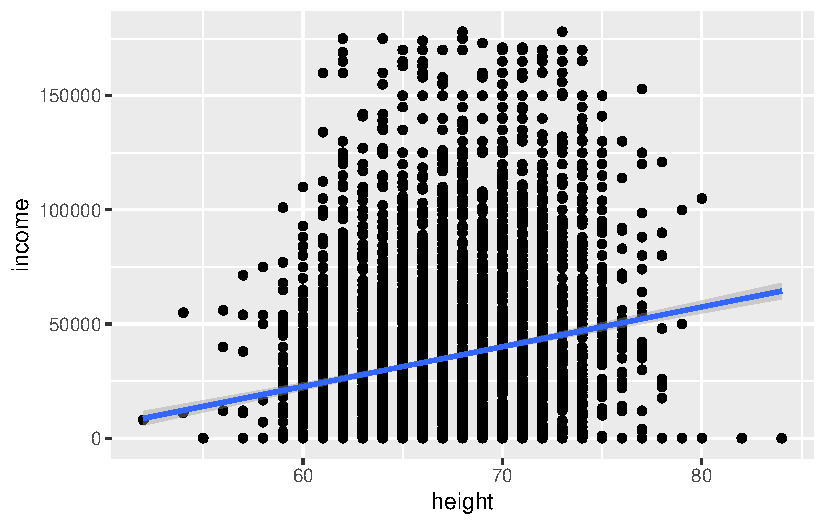
\includegraphics{EDA_files/figure-pdf/unnamed-chunk-3-1.pdf}

}

\end{figure}

\begin{Shaded}
\begin{Highlighting}[]
\FunctionTok{summary}\NormalTok{(heights)}
\end{Highlighting}
\end{Shaded}

\begin{verbatim}
     income             height         weight           age       
 Min.   :     0.0   Min.   :52.0   Min.   : 76.0   Min.   :47.00  
 1st Qu.:   165.5   1st Qu.:64.0   1st Qu.:157.0   1st Qu.:49.00  
 Median : 29589.5   Median :67.0   Median :184.0   Median :51.00  
 Mean   : 41203.9   Mean   :67.1   Mean   :188.3   Mean   :51.33  
 3rd Qu.: 55000.0   3rd Qu.:70.0   3rd Qu.:212.0   3rd Qu.:53.00  
 Max.   :343830.0   Max.   :84.0   Max.   :524.0   Max.   :56.00  
                                   NA's   :95                     
      marital         sex         education          afqt       
 single   :1124   male  :3402   Min.   : 1.00   Min.   :  0.00  
 married  :3806   female:3604   1st Qu.:12.00   1st Qu.: 15.12  
 separated: 366                 Median :12.00   Median : 36.76  
 divorced :1549                 Mean   :13.22   Mean   : 41.21  
 widowed  : 161                 3rd Qu.:15.00   3rd Qu.: 65.24  
                                Max.   :20.00   Max.   :100.00  
                                NA's   :10      NA's   :262     
\end{verbatim}

\hypertarget{na-i-heights}{%
\subsection{NA i heights:}\label{na-i-heights}}

\begin{Shaded}
\begin{Highlighting}[]
\CommentTok{\# NAs in heights?}
\NormalTok{heights }\SpecialCharTok{\%\textgreater{}\%} 
  \FunctionTok{apply}\NormalTok{(}\AttributeTok{MARGIN =} \DecValTok{2}\NormalTok{, }\AttributeTok{FUN =}\NormalTok{ is.na) }\SpecialCharTok{\%\textgreater{}\%} 
  \FunctionTok{apply}\NormalTok{(}\AttributeTok{MARGIN =} \DecValTok{2}\NormalTok{, }\AttributeTok{FUN =}\NormalTok{ sum) }
\end{Highlighting}
\end{Shaded}

\begin{verbatim}
   income    height    weight       age   marital       sex education      afqt 
        0         0        95         0         0         0        10       262 
\end{verbatim}

Får akkurat samme svar ved å bruke komandoen:

\begin{Shaded}
\begin{Highlighting}[]
\CommentTok{\# NAs in heights?}
\NormalTok{heights }\SpecialCharTok{\%\textgreater{}\%} 
  \FunctionTok{is.na}\NormalTok{() }\SpecialCharTok{\%\textgreater{}\%} 
  \FunctionTok{apply}\NormalTok{(}\AttributeTok{MARGIN =} \DecValTok{2}\NormalTok{, }\AttributeTok{FUN =}\NormalTok{ sum) }
\end{Highlighting}
\end{Shaded}

\begin{verbatim}
   income    height    weight       age   marital       sex education      afqt 
        0         0        95         0         0         0        10       262 
\end{verbatim}

Her får vi bare opp de variablene som faktisk har NA verdier.

\begin{itemize}
\tightlist
\item
  Punktum betyr her dataene i pipen. Legger det inn i firkanklammer for
  å gi beskjed om hvilke verdier jeg vil ha med fra dataframen.
\end{itemize}

\begin{Shaded}
\begin{Highlighting}[]
\CommentTok{\# number of NAs in each variable}
\CommentTok{\# drop variables with no NA}
\NormalTok{heights }\SpecialCharTok{\%\textgreater{}\%} 
  \FunctionTok{is.na}\NormalTok{() }\SpecialCharTok{\%\textgreater{}\%} 
  \FunctionTok{colSums}\NormalTok{() }\SpecialCharTok{\%\textgreater{}\%} 
\NormalTok{  .[. }\SpecialCharTok{\textgreater{}} \DecValTok{0}\NormalTok{]}
\end{Highlighting}
\end{Shaded}

\begin{verbatim}
   weight education      afqt 
       95        10       262 
\end{verbatim}

\hypertarget{vtable---pakke}{%
\subsection{Vtable - pakke}\label{vtable---pakke}}

\hypertarget{summary-statistics}{%
\subsubsection{Summary Statistics}\label{summary-statistics}}

Her tar vi ikke med variablene ``marital og sex''

\begin{itemize}
\tightlist
\item
  St gir oss tabellen i viewer
\end{itemize}

\begin{Shaded}
\begin{Highlighting}[]
\CommentTok{\# package vtable must be installed}
\NormalTok{heights }\SpecialCharTok{\%\textgreater{}\%} 
  \FunctionTok{select}\NormalTok{(}\SpecialCharTok{{-}}\NormalTok{marital, }\SpecialCharTok{{-}}\NormalTok{sex) }\SpecialCharTok{\%\textgreater{}\%} 
\NormalTok{  vtable}\SpecialCharTok{::}\FunctionTok{st}\NormalTok{()}
\end{Highlighting}
\end{Shaded}

\begin{table}

\caption{Summary Statistics}
\centering
\begin{tabular}[t]{llllllll}
\toprule
Variable & N & Mean & Std. Dev. & Min & Pctl. 25 & Pctl. 75 & Max\\
\midrule
income & 7006 & 41204 & 55892 & 0 & 166 & 55000 & 343830\\
height & 7006 & 67 & 4.1 & 52 & 64 & 70 & 84\\
weight & 6911 & 188 & 44 & 76 & 157 & 212 & 524\\
age & 7006 & 51 & 2.2 & 47 & 49 & 53 & 56\\
education & 6996 & 13 & 2.6 & 1 & 12 & 15 & 20\\
\addlinespace
afqt & 6744 & 41 & 29 & 0 & 15 & 65 & 100\\
\bottomrule
\end{tabular}
\end{table}

Her får vi bare opp variablene ``marital og sex''

\begin{Shaded}
\begin{Highlighting}[]
\CommentTok{\# package vtable must be installed}
\NormalTok{heights }\SpecialCharTok{\%\textgreater{}\%} 
  \FunctionTok{select}\NormalTok{(marital, sex) }\SpecialCharTok{\%\textgreater{}\%} 
\NormalTok{  vtable}\SpecialCharTok{::}\FunctionTok{st}\NormalTok{(.)}
\end{Highlighting}
\end{Shaded}

\begin{table}

\caption{Summary Statistics}
\centering
\begin{tabular}[t]{lll}
\toprule
Variable & N & Percent\\
\midrule
marital & 7006 & \\
... single & 1124 & 16%\\
... married & 3806 & 54%\\
... separated & 366 & 5%\\
... divorced & 1549 & 22%\\
\addlinespace
... widowed & 161 & 2%\\
sex & 7006 & \\
... male & 3402 & 49%\\
... female & 3604 & 51%\\
\bottomrule
\end{tabular}
\end{table}

\textbf{Så ønsker vi å se litt nærmere på sivilstatus (marital):}

\begin{enumerate}
\def\labelenumi{\arabic{enumi}.}
\tightlist
\item
  Først dropper vi sivilstatus og lager en tabell som blir fordelt
  mellom menn og kvinner:
\end{enumerate}

\begin{Shaded}
\begin{Highlighting}[]
\NormalTok{heights }\SpecialCharTok{\%\textgreater{}\%} 
  \FunctionTok{select}\NormalTok{(}\SpecialCharTok{{-}}\NormalTok{marital) }\SpecialCharTok{\%\textgreater{}\%} 
\NormalTok{  vtable}\SpecialCharTok{::}\FunctionTok{st}\NormalTok{(}\AttributeTok{group =} \StringTok{\textquotesingle{}sex\textquotesingle{}}\NormalTok{)}
\end{Highlighting}
\end{Shaded}

\begin{table}

\caption{Summary Statistics}
\centering
\begin{tabular}[t]{lllllll}
\toprule
\multicolumn{1}{c}{sex} & \multicolumn{3}{c}{male} & \multicolumn{3}{c}{female} \\
\cmidrule(l{3pt}r{3pt}){1-1} \cmidrule(l{3pt}r{3pt}){2-4} \cmidrule(l{3pt}r{3pt}){5-7}
Variable & N & Mean & SD & N & Mean & SD\\
\midrule
income & 3402 & 53510 & 69399 & 3604 & 29588 & 35347\\
height & 3402 & 70 & 3 & 3604 & 64 & 2.7\\
weight & 3392 & 204 & 41 & 3519 & 173 & 43\\
age & 3402 & 51 & 2.2 & 3604 & 51 & 2.2\\
education & 3396 & 13 & 2.6 & 3600 & 13 & 2.6\\
\addlinespace
afqt & 3248 & 42 & 30 & 3496 & 41 & 28\\
\bottomrule
\end{tabular}
\end{table}

Her gjør vi en liten bearbeidelse i sivilstatus varaiabelen. Marital
inneholdt 5 ulike kategorier -\textgreater{} gift, ugift, skilt, enke og
separert.

Lager en ny variabel som heter gift, og skille denne på - \textbf{gift
eller ikke gift}. Vi går fra å ha 5 kategorier til å bruke true og false
til å svare på om du er gift eller ikke.

Siden vi lager oss en ny variabel ``married'' bruker vi komandoen
``mutate''

Videre vil jeg bare se på \textbf{kvinnene}, og derfor dropper jeg
variabelen ``sex''.

\begin{Shaded}
\begin{Highlighting}[]
\CommentTok{\# package vtable must be installed}
\NormalTok{heights }\SpecialCharTok{\%\textgreater{}\%} 
  \FunctionTok{mutate}\NormalTok{(}
    \AttributeTok{married =} \FunctionTok{if\_else}\NormalTok{(}
\NormalTok{    marital }\SpecialCharTok{==} \StringTok{\textquotesingle{}married\textquotesingle{}}\NormalTok{, }
    \ConstantTok{TRUE}\NormalTok{,}
    \ConstantTok{FALSE}
\NormalTok{    )}
\NormalTok{  ) }\SpecialCharTok{\%\textgreater{}\%} 
  \FunctionTok{filter}\NormalTok{(sex }\SpecialCharTok{==} \StringTok{\textquotesingle{}female\textquotesingle{}}\NormalTok{) }\SpecialCharTok{\%\textgreater{}\%} 
  \FunctionTok{select}\NormalTok{(}\SpecialCharTok{{-}}\NormalTok{sex, }\SpecialCharTok{{-}}\NormalTok{marital) }\SpecialCharTok{\%\textgreater{}\%} 
\NormalTok{  vtable}\SpecialCharTok{::}\FunctionTok{st}\NormalTok{(}\AttributeTok{group =} \StringTok{\textquotesingle{}married\textquotesingle{}}\NormalTok{)}
\end{Highlighting}
\end{Shaded}

\begin{table}

\caption{Summary Statistics}
\centering
\begin{tabular}[t]{lllllll}
\toprule
\multicolumn{1}{c}{married} & \multicolumn{3}{c}{No} & \multicolumn{3}{c}{Yes} \\
\cmidrule(l{3pt}r{3pt}){1-1} \cmidrule(l{3pt}r{3pt}){2-4} \cmidrule(l{3pt}r{3pt}){5-7}
Variable & N & Mean & SD & N & Mean & SD\\
\midrule
income & 1703 & 26682 & 30962 & 1901 & 32190 & 38680\\
height & 1703 & 64 & 2.8 & 1901 & 64 & 2.7\\
weight & 1662 & 177 & 45 & 1857 & 169 & 40\\
age & 1703 & 51 & 2.3 & 1901 & 51 & 2.2\\
education & 1701 & 13 & 2.6 & 1899 & 14 & 2.6\\
\addlinespace
afqt & 1647 & 33 & 26 & 1849 & 47 & 28\\
\bottomrule
\end{tabular}
\end{table}

Så vil vi se på \textbf{mennene}:

\begin{Shaded}
\begin{Highlighting}[]
\CommentTok{\# package vtable must be installed}
\NormalTok{heights }\SpecialCharTok{\%\textgreater{}\%} 
  \FunctionTok{mutate}\NormalTok{(}
    \AttributeTok{married =} \FunctionTok{if\_else}\NormalTok{(}
\NormalTok{    marital }\SpecialCharTok{==} \StringTok{\textquotesingle{}married\textquotesingle{}}\NormalTok{, }
    \ConstantTok{TRUE}\NormalTok{,}
    \ConstantTok{FALSE}
\NormalTok{    )}
\NormalTok{  ) }\SpecialCharTok{\%\textgreater{}\%} 
  \FunctionTok{filter}\NormalTok{(sex }\SpecialCharTok{==} \StringTok{\textquotesingle{}male\textquotesingle{}}\NormalTok{) }\SpecialCharTok{\%\textgreater{}\%} 
  \FunctionTok{select}\NormalTok{(}\SpecialCharTok{{-}}\NormalTok{sex, }\SpecialCharTok{{-}}\NormalTok{marital) }\SpecialCharTok{\%\textgreater{}\%} 
\NormalTok{  vtable}\SpecialCharTok{::}\FunctionTok{st}\NormalTok{(}\AttributeTok{group =} \StringTok{\textquotesingle{}married\textquotesingle{}}\NormalTok{)}
\end{Highlighting}
\end{Shaded}

\begin{table}

\caption{Summary Statistics}
\centering
\begin{tabular}[t]{lllllll}
\toprule
\multicolumn{1}{c}{married} & \multicolumn{3}{c}{No} & \multicolumn{3}{c}{Yes} \\
\cmidrule(l{3pt}r{3pt}){1-1} \cmidrule(l{3pt}r{3pt}){2-4} \cmidrule(l{3pt}r{3pt}){5-7}
Variable & N & Mean & SD & N & Mean & SD\\
\midrule
income & 1497 & 32122 & 50520 & 1905 & 70317 & 77171\\
height & 1497 & 70 & 3.1 & 1905 & 70 & 2.9\\
weight & 1492 & 200 & 42 & 1900 & 207 & 39\\
age & 1497 & 51 & 2.2 & 1905 & 51 & 2.3\\
education & 1494 & 12 & 2.2 & 1902 & 14 & 2.7\\
\addlinespace
afqt & 1426 & 34 & 28 & 1822 & 48 & 30\\
\bottomrule
\end{tabular}
\end{table}

\hypertarget{grafisk-greie-puxe5-en-variabel}{%
\subsection{Grafisk greie på en
variabel}\label{grafisk-greie-puxe5-en-variabel}}

\begin{Shaded}
\begin{Highlighting}[]
\FunctionTok{ggplot}\NormalTok{(}\AttributeTok{data =}\NormalTok{ heights) }\SpecialCharTok{+}
  \FunctionTok{geom\_bar}\NormalTok{(}\AttributeTok{mapping =} \FunctionTok{aes}\NormalTok{(}\AttributeTok{x =}\NormalTok{ education), }\AttributeTok{na.rm =} \ConstantTok{TRUE}\NormalTok{)}
\end{Highlighting}
\end{Shaded}

\begin{figure}[H]

{\centering 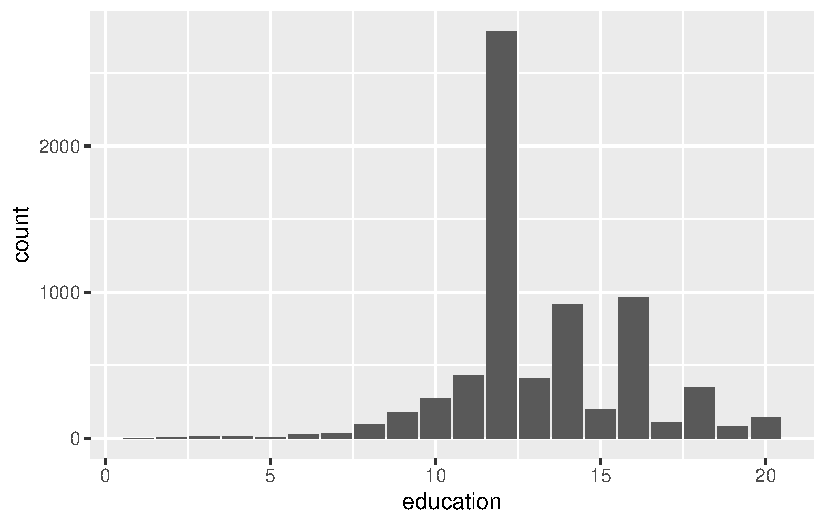
\includegraphics{EDA_files/figure-pdf/unnamed-chunk-13-1.pdf}

}

\end{figure}

\begin{Shaded}
\begin{Highlighting}[]
\NormalTok{hist1 }\OtherTok{\textless{}{-}}\NormalTok{ ggplotify}\SpecialCharTok{::}\FunctionTok{as.ggplot}\NormalTok{(}\SpecialCharTok{\textasciitilde{}}\FunctionTok{hist}\NormalTok{(heights}\SpecialCharTok{$}\NormalTok{income, }\AttributeTok{breaks =} \DecValTok{20}\NormalTok{))}
\NormalTok{hist2 }\OtherTok{\textless{}{-}} \FunctionTok{ggplot}\NormalTok{(heights, }\AttributeTok{mapping =} \FunctionTok{aes}\NormalTok{(}\AttributeTok{x =}\NormalTok{ income)) }\SpecialCharTok{+}
  \FunctionTok{geom\_histogram}\NormalTok{(}\AttributeTok{bins =} \DecValTok{20}\NormalTok{)}

\NormalTok{gridExtra}\SpecialCharTok{::}\FunctionTok{grid.arrange}\NormalTok{(hist1, hist2, }\AttributeTok{ncol =} \DecValTok{2}\NormalTok{)}
\end{Highlighting}
\end{Shaded}

\begin{figure}[H]

{\centering 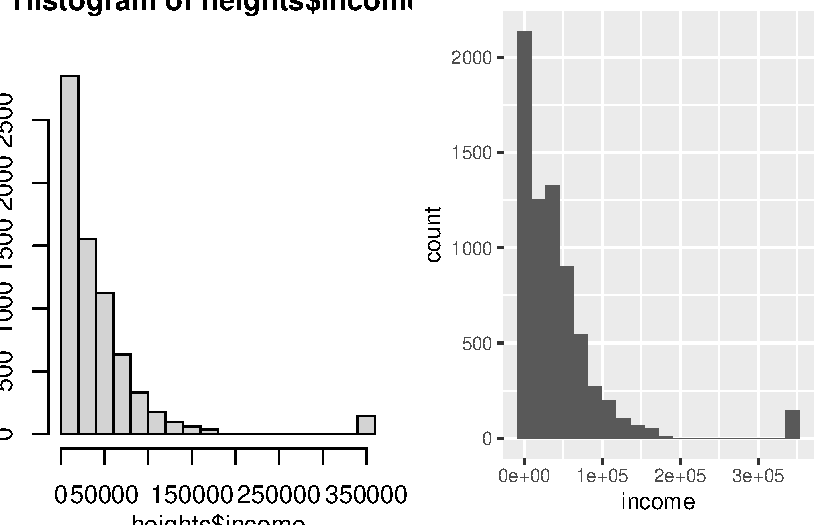
\includegraphics{EDA_files/figure-pdf/unnamed-chunk-14-1.pdf}

}

\end{figure}

Her bruker vi log (logaritme)

\begin{Shaded}
\begin{Highlighting}[]
\NormalTok{hist1 }\OtherTok{\textless{}{-}}\NormalTok{ ggplotify}\SpecialCharTok{::}\FunctionTok{as.ggplot}\NormalTok{(}\SpecialCharTok{\textasciitilde{}}\FunctionTok{hist}\NormalTok{(}\FunctionTok{log}\NormalTok{(heights}\SpecialCharTok{$}\NormalTok{income }\SpecialCharTok{+} \DecValTok{1}\NormalTok{), }\AttributeTok{breaks =} \DecValTok{20}\NormalTok{))}
\NormalTok{hist2 }\OtherTok{\textless{}{-}} \FunctionTok{ggplot}\NormalTok{(heights, }\AttributeTok{mapping =} \FunctionTok{aes}\NormalTok{(}\AttributeTok{x =} \FunctionTok{log}\NormalTok{(income }\SpecialCharTok{+} \DecValTok{1}\NormalTok{)))}\SpecialCharTok{+}
  \FunctionTok{geom\_histogram}\NormalTok{(}\AttributeTok{bins =} \DecValTok{20}\NormalTok{)}

\NormalTok{gridExtra}\SpecialCharTok{::}\FunctionTok{grid.arrange}\NormalTok{(hist1, hist2, }\AttributeTok{ncol =} \DecValTok{2}\NormalTok{)}
\end{Highlighting}
\end{Shaded}

\begin{figure}[H]

{\centering 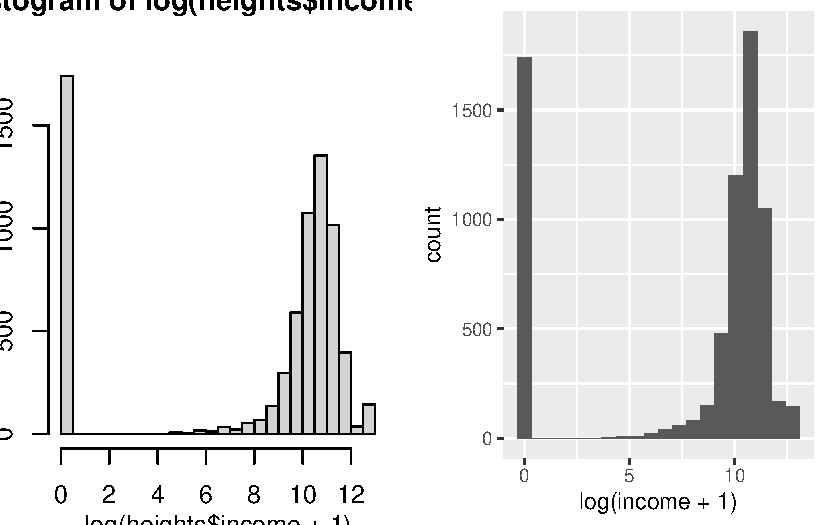
\includegraphics{EDA_files/figure-pdf/unnamed-chunk-15-1.pdf}

}

\end{figure}

Generere tre ulike historgram for tre ulike variabler -\textgreater{}
income, height og weight

\begin{Shaded}
\begin{Highlighting}[]
\NormalTok{hist3 }\OtherTok{\textless{}{-}} \FunctionTok{ggplot}\NormalTok{(heights, }\AttributeTok{mapping =} \FunctionTok{aes}\NormalTok{(}\AttributeTok{x =}\NormalTok{ income)) }\SpecialCharTok{+}
  \FunctionTok{geom\_histogram}\NormalTok{(}\AttributeTok{bins =} \DecValTok{40}\NormalTok{, }\AttributeTok{na.rm =} \ConstantTok{TRUE}\NormalTok{)}
\NormalTok{hist4 }\OtherTok{\textless{}{-}} \FunctionTok{ggplot}\NormalTok{(heights, }\AttributeTok{mapping =} \FunctionTok{aes}\NormalTok{(}\AttributeTok{x =}\NormalTok{ height)) }\SpecialCharTok{+}
  \FunctionTok{geom\_histogram}\NormalTok{(}\AttributeTok{bins =} \DecValTok{40}\NormalTok{, }\AttributeTok{na.rm =} \ConstantTok{TRUE}\NormalTok{)}
\NormalTok{hist5 }\OtherTok{\textless{}{-}} \FunctionTok{ggplot}\NormalTok{(heights, }\AttributeTok{mapping =} \FunctionTok{aes}\NormalTok{(}\AttributeTok{x =}\NormalTok{ weight)) }\SpecialCharTok{+}
  \FunctionTok{geom\_histogram}\NormalTok{(}\AttributeTok{bins =} \DecValTok{40}\NormalTok{, }\AttributeTok{na.rm =} \ConstantTok{TRUE}\NormalTok{)}
\NormalTok{gridExtra}\SpecialCharTok{::}\FunctionTok{grid.arrange}\NormalTok{(hist3, hist4, hist5, }\AttributeTok{nrow =} \DecValTok{1}\NormalTok{)}
\end{Highlighting}
\end{Shaded}

\begin{figure}[H]

{\centering 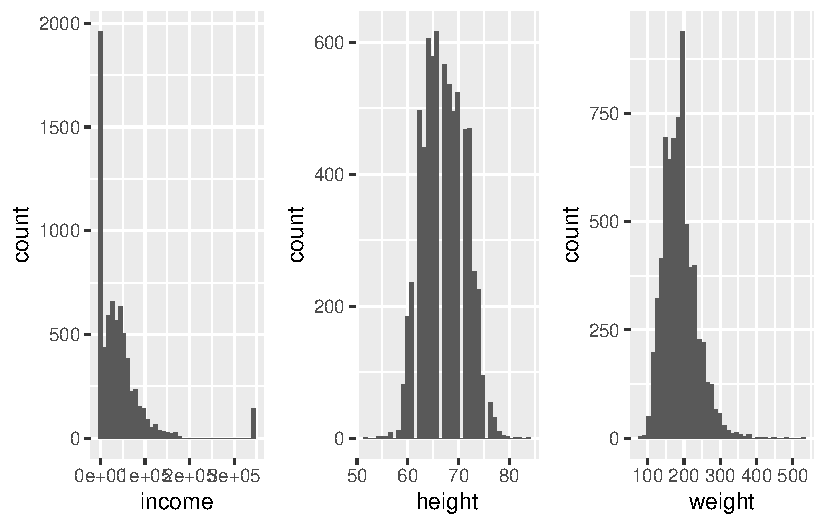
\includegraphics{EDA_files/figure-pdf/unnamed-chunk-16-1.pdf}

}

\end{figure}

\begin{Shaded}
\begin{Highlighting}[]
\NormalTok{hist6 }\OtherTok{\textless{}{-}} \FunctionTok{ggplot}\NormalTok{(heights, }\AttributeTok{mapping =} \FunctionTok{aes}\NormalTok{(}\AttributeTok{x =}\NormalTok{ age)) }\SpecialCharTok{+}
  \FunctionTok{geom\_histogram}\NormalTok{(}\AttributeTok{bins =} \DecValTok{40}\NormalTok{, }\AttributeTok{na.rm =} \ConstantTok{TRUE}\NormalTok{)}
\NormalTok{hist7 }\OtherTok{\textless{}{-}} \FunctionTok{ggplot}\NormalTok{(heights, }\AttributeTok{mapping =} \FunctionTok{aes}\NormalTok{(}\AttributeTok{x =}\NormalTok{ education)) }\SpecialCharTok{+}
  \FunctionTok{geom\_histogram}\NormalTok{(}\AttributeTok{bins =} \DecValTok{40}\NormalTok{, }\AttributeTok{na.rm =} \ConstantTok{TRUE}\NormalTok{)}
\NormalTok{hist8 }\OtherTok{\textless{}{-}} \FunctionTok{ggplot}\NormalTok{(heights, }\AttributeTok{mapping =} \FunctionTok{aes}\NormalTok{(}\AttributeTok{x =}\NormalTok{ afqt)) }\SpecialCharTok{+}
  \FunctionTok{geom\_histogram}\NormalTok{(}\AttributeTok{bins =} \DecValTok{40}\NormalTok{, }\AttributeTok{na.rm =} \ConstantTok{TRUE}\NormalTok{)}
\NormalTok{gridExtra}\SpecialCharTok{::}\FunctionTok{grid.arrange}\NormalTok{(hist6, hist7, hist8, }\AttributeTok{nrow =} \DecValTok{1}\NormalTok{)}
\end{Highlighting}
\end{Shaded}

\begin{figure}[H]

{\centering 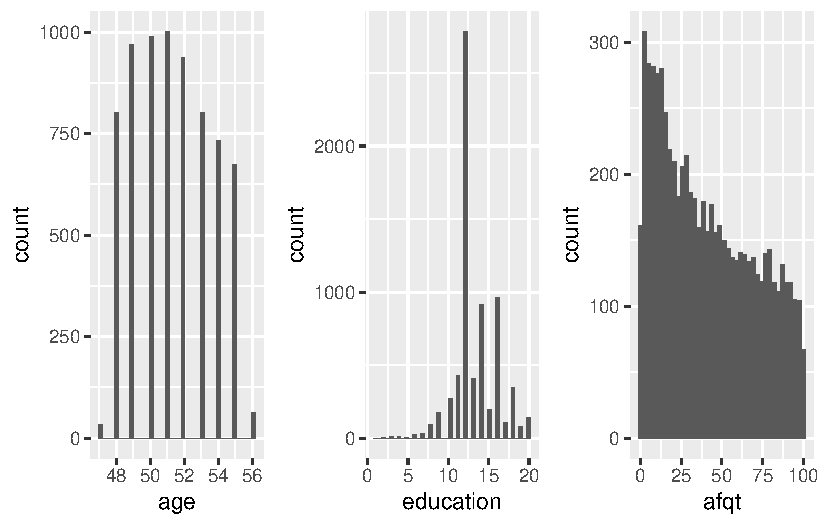
\includegraphics{EDA_files/figure-pdf/unnamed-chunk-17-1.pdf}

}

\end{figure}

\hypertarget{geom_density}{%
\subsection{\texorpdfstring{\texttt{geom\_density()}}{geom\_density()}}\label{geom_density}}

Disse kurvene er greit å bruke til å se på forskjeller i datasette. Man
kan også bruke historgram men disse density kurvene er bedre.

Denne viser de som \textbf{ikke} har fullført HS(high school'', de som
ikke har fulført TC osv\ldots{}

\begin{Shaded}
\begin{Highlighting}[]
\NormalTok{heights }\SpecialCharTok{\%\textgreater{}\%} 
  \FunctionTok{mutate}\NormalTok{(}
    \AttributeTok{edu\_fac =} \FunctionTok{cut}\NormalTok{(education, }
                  \AttributeTok{breaks =} \FunctionTok{c}\NormalTok{(}\DecValTok{0}\NormalTok{, }\DecValTok{12}\NormalTok{, }\DecValTok{14}\NormalTok{, }\DecValTok{16}\NormalTok{, }\DecValTok{21}\NormalTok{), }
                  \AttributeTok{labels =} \FunctionTok{c}\NormalTok{(}\StringTok{"NotHS"}\NormalTok{, }\StringTok{"NotTC"}\NormalTok{, }\StringTok{"NotC"}\NormalTok{, }\StringTok{"C+"}\NormalTok{),}
                  \AttributeTok{right =} \ConstantTok{FALSE}\NormalTok{) }
\NormalTok{  ) }\SpecialCharTok{\%\textgreater{}\%} 
  \FunctionTok{filter}\NormalTok{(}\SpecialCharTok{!}\FunctionTok{is.na}\NormalTok{(edu\_fac) }\SpecialCharTok{\&}\NormalTok{ income }\SpecialCharTok{\textgreater{}} \DecValTok{0}\NormalTok{) }\SpecialCharTok{\%\textgreater{}\%}
  \FunctionTok{ggplot}\NormalTok{(}\AttributeTok{mapping =} \FunctionTok{aes}\NormalTok{(}\AttributeTok{x =}\NormalTok{ income, }\AttributeTok{fill =}\NormalTok{ edu\_fac, }\AttributeTok{colour =}\NormalTok{ edu\_fac)) }\SpecialCharTok{+}
  \FunctionTok{geom\_density}\NormalTok{(}\AttributeTok{alpha =} \FloatTok{0.2}\NormalTok{, }\AttributeTok{na.rm =} \ConstantTok{TRUE}\NormalTok{) }\SpecialCharTok{+} 
  \FunctionTok{facet\_wrap}\NormalTok{(}\SpecialCharTok{\textasciitilde{}}\NormalTok{sex)}
\end{Highlighting}
\end{Shaded}

\begin{figure}[H]

{\centering 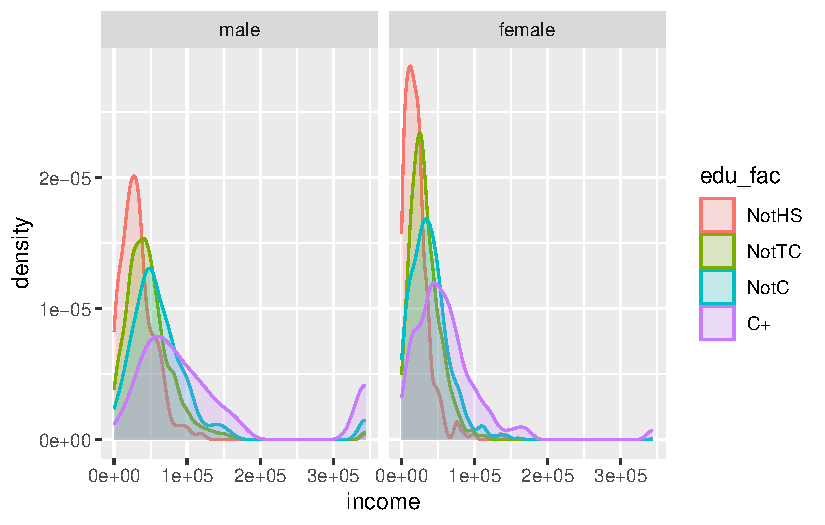
\includegraphics{EDA_files/figure-pdf/unnamed-chunk-18-1.pdf}

}

\end{figure}

\begin{Shaded}
\begin{Highlighting}[]
\NormalTok{heights }\SpecialCharTok{\%\textgreater{}\%} 
  \FunctionTok{mutate}\NormalTok{(}
    \AttributeTok{edu\_fac =} \FunctionTok{cut}\NormalTok{(education, }
                  \AttributeTok{breaks =} \FunctionTok{c}\NormalTok{(}\DecValTok{0}\NormalTok{, }\DecValTok{12}\NormalTok{, }\DecValTok{14}\NormalTok{, }\DecValTok{16}\NormalTok{, }\DecValTok{21}\NormalTok{), }
                  \AttributeTok{labels =} \FunctionTok{c}\NormalTok{(}\StringTok{"NotHS"}\NormalTok{, }\StringTok{"NotTC"}\NormalTok{, }\StringTok{"NotC"}\NormalTok{, }\StringTok{"C+"}\NormalTok{),}
                  \AttributeTok{right =} \ConstantTok{FALSE}\NormalTok{) }
\NormalTok{  ) }\SpecialCharTok{\%\textgreater{}\%} 
  \FunctionTok{filter}\NormalTok{(}\SpecialCharTok{!}\FunctionTok{is.na}\NormalTok{(edu\_fac) }\SpecialCharTok{\&}\NormalTok{ income }\SpecialCharTok{\textgreater{}} \DecValTok{0}  \SpecialCharTok{\&}\NormalTok{ income }\SpecialCharTok{\textless{}} \DecValTok{250000}\NormalTok{) }\SpecialCharTok{\%\textgreater{}\%}
  \FunctionTok{ggplot}\NormalTok{(}\AttributeTok{mapping =} \FunctionTok{aes}\NormalTok{(}\AttributeTok{x =}\NormalTok{ income, }\AttributeTok{fill =}\NormalTok{ edu\_fac, }\AttributeTok{colour =}\NormalTok{ edu\_fac)) }\SpecialCharTok{+}
  \FunctionTok{geom\_density}\NormalTok{(}\AttributeTok{alpha =} \FloatTok{0.2}\NormalTok{, }\AttributeTok{na.rm =} \ConstantTok{TRUE}\NormalTok{) }\SpecialCharTok{+} 
  \FunctionTok{facet\_wrap}\NormalTok{(}\SpecialCharTok{\textasciitilde{}}\NormalTok{sex)}
\end{Highlighting}
\end{Shaded}

\begin{figure}[H]

{\centering 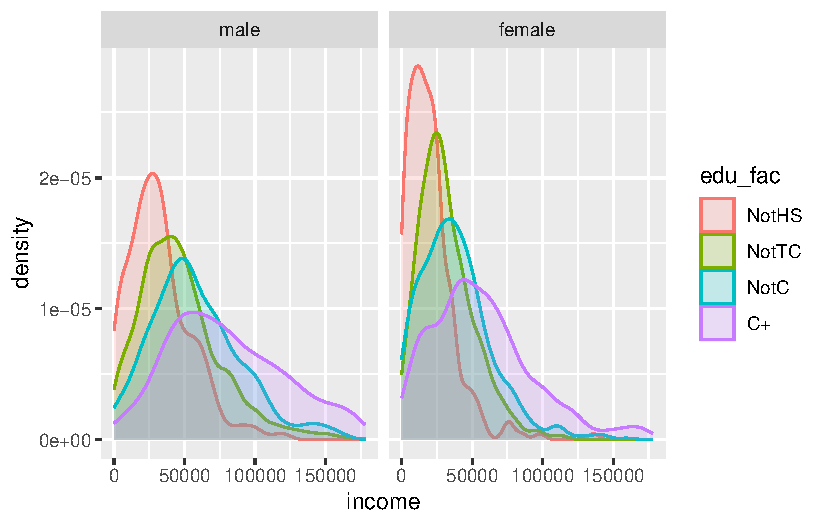
\includegraphics{EDA_files/figure-pdf/unnamed-chunk-19-1.pdf}

}

\end{figure}

Her er de samme dataene illustrert på en annen måte. Her er de
illustrert ved hjelp av 4 plott men med to density - en for menn og en
for kvinner:

\begin{Shaded}
\begin{Highlighting}[]
\NormalTok{heights }\SpecialCharTok{\%\textgreater{}\%} 
  \FunctionTok{mutate}\NormalTok{(}
    \AttributeTok{edu\_fac =} \FunctionTok{cut}\NormalTok{(education, }
                  \AttributeTok{breaks =} \FunctionTok{c}\NormalTok{(}\DecValTok{0}\NormalTok{, }\DecValTok{12}\NormalTok{, }\DecValTok{14}\NormalTok{, }\DecValTok{16}\NormalTok{, }\DecValTok{21}\NormalTok{), }
                  \AttributeTok{labels =} \FunctionTok{c}\NormalTok{(}\StringTok{"NotHS"}\NormalTok{, }\StringTok{"NotTC"}\NormalTok{, }\StringTok{"NotC"}\NormalTok{, }\StringTok{"C+"}\NormalTok{),}
                  \AttributeTok{right =} \ConstantTok{FALSE}\NormalTok{) }
\NormalTok{  ) }\SpecialCharTok{\%\textgreater{}\%} 
  \FunctionTok{filter}\NormalTok{(}\SpecialCharTok{!}\FunctionTok{is.na}\NormalTok{(edu\_fac) }\SpecialCharTok{\&}\NormalTok{ income }\SpecialCharTok{\textgreater{}} \DecValTok{0}\NormalTok{) }\SpecialCharTok{\%\textgreater{}\%}
  \FunctionTok{ggplot}\NormalTok{(}\AttributeTok{mapping =} \FunctionTok{aes}\NormalTok{(}\AttributeTok{x =}\NormalTok{ income, }\AttributeTok{fill =}\NormalTok{ sex, }\AttributeTok{colour =}\NormalTok{ sex)) }\SpecialCharTok{+}
  \FunctionTok{geom\_density}\NormalTok{(}\AttributeTok{alpha =} \FloatTok{0.2}\NormalTok{, }\AttributeTok{na.rm =} \ConstantTok{TRUE}\NormalTok{) }\SpecialCharTok{+} 
  \FunctionTok{facet\_wrap}\NormalTok{(}\SpecialCharTok{\textasciitilde{}}\NormalTok{edu\_fac)}
\end{Highlighting}
\end{Shaded}

\begin{figure}[H]

{\centering 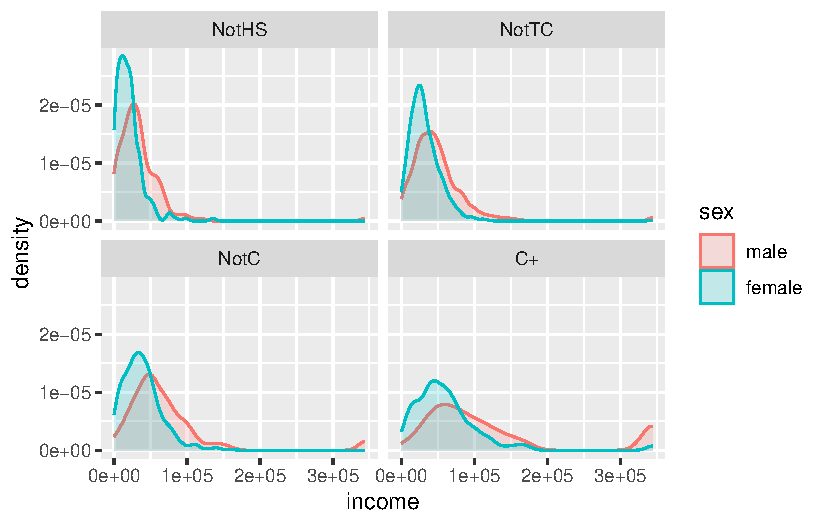
\includegraphics{EDA_files/figure-pdf/unnamed-chunk-20-1.pdf}

}

\end{figure}



\end{document}
